%!TEX root = ../../../main.tex

	\subsection{Sideband} \label{subsubsec::sideband}

		It is known that the \pl spectra of \sivs in \nd are dominated by the \zpl. As a result \psb contributions remain small, a fact expressed in large \db factors of over \SI{70}{\percent} established previously \cite{Neu2011,Neu2011b}. Our own measurements are consistent with these of \emnarrow and \embroad results. We also find distinct sideband peaks in many \siv \pl emission spectra.
		The investigated emitters exhibit two different structures of sideband spectra: The spectra in \vl exhibit one strong sideband peak, spectra in \hl exhibit several weaker sideband peaks. \Fref{subfig::sideband_group_v} and \Fref{subfig::sideband_group_h} illustrate the respective observations.

		\begin{figure}[!htb]
			\begin{subfigure}{0.49\linewidth}
				\centering
				\testbox{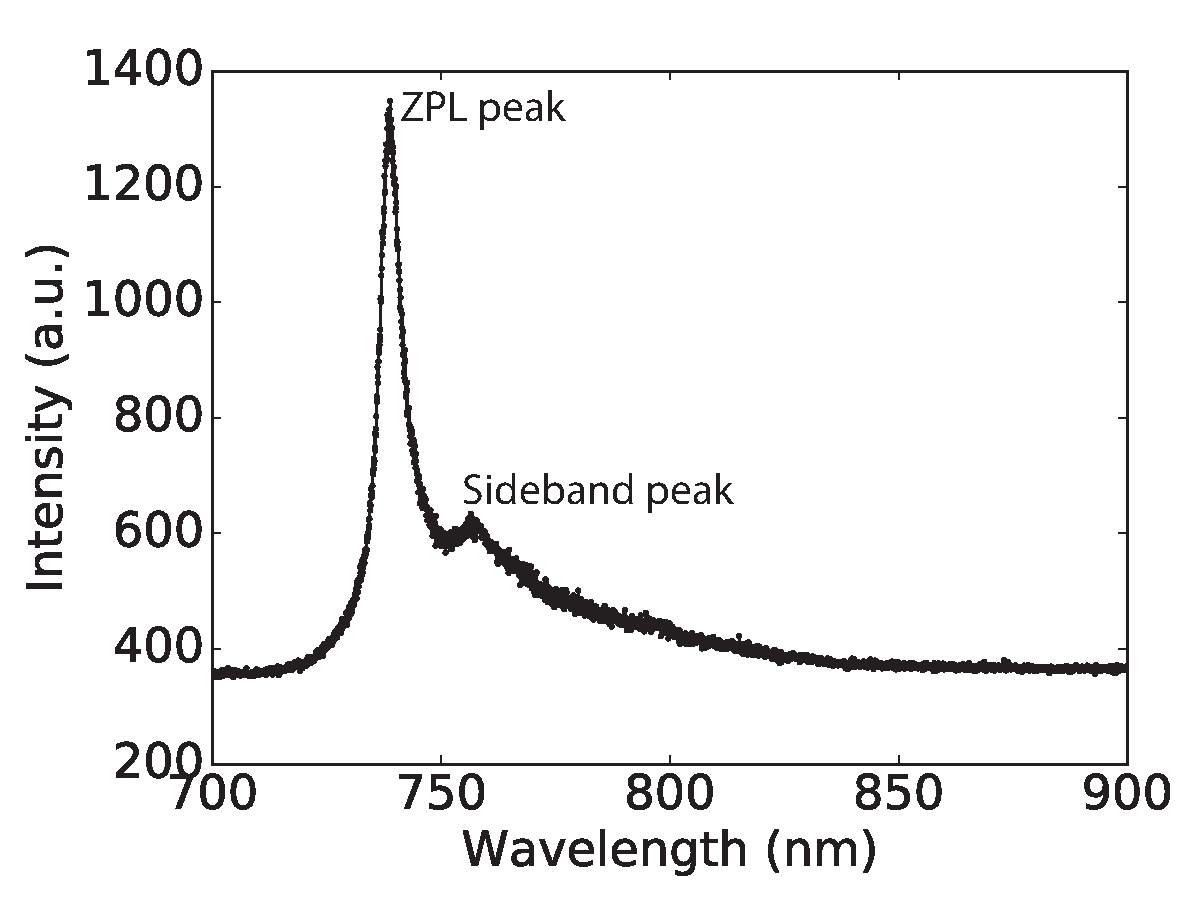
\includegraphics[trim = 0 0 0 0,  clip= true, width = \pairplotwide]{./pics/Ir25M_spe_scan_xy-38x9y16_300uW_t120.pdf}}
				\caption{}
				\label{subfig::sideband_group_v}
			\end{subfigure}
			\hfill
			\begin{subfigure}{0.49\linewidth}
				\centering
				\testbox{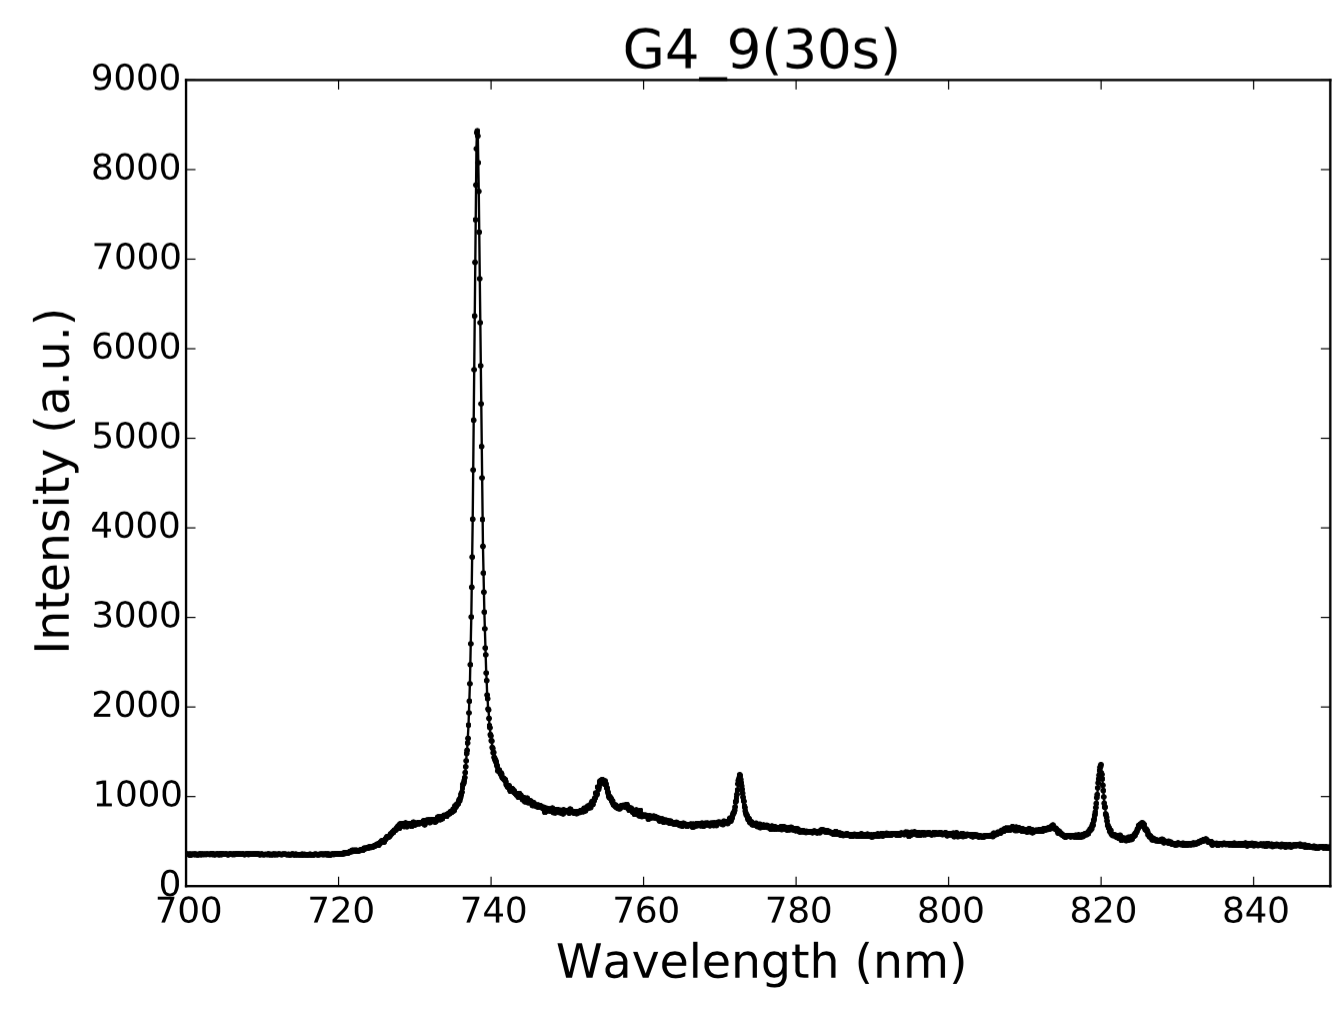
\includegraphics[trim = 0 0 0 0,  clip= true, width = \pairplotwide]{./pics/G4_9_30s.png}}
				\caption{}
				\label{subfig::sideband_group_h}
			\end{subfigure}
			\caption[Side band peaks for \sivs]{Representative spectra of emitters showing single (\subref{subfig::sideband_group_v}) and multiple (\subref{subfig::sideband_group_h}) side band peaks. The former belong to \vl, while the latter are members of \hl.}
			\label{fig::sideband_groups}
		\end{figure}

		Most of the spectra in \vl exhibit a characteristic shape, composed of the \ZPL and one strong sideband peak.
		\SI{70}{\percent} of the \pl spectra with one distinct sideband peak exhibit a shift of the sideband peak from the \ZPL between \SIrange{37}{43}{meV}.
		The range of line shifts for the prominent sideband peak coincides with a well-known feature at \SI{42}{meV}, associated with \sivs \cite{Larkins1971,Sternschulte1994}, but also to a larger number of optically active defects \cite{Sternschulte1994}.
		The occurrence of this \SI{42}{meV} sideband feature for a large number of defects and the absence of isotopic variations \cite{Dietrich2014}, favors an assignment as non-localized lattice vibration.
		We furthermore observe that the dominant sideband peak shifts towards smaller distance from the \ZPL for increasing \ZPL \cwl, i.e.\ increasing strain. \Fref{fig::sideband_fit} presents a linear fit to data for emitters in \vl..
		The low phonon energy of the sideband feature and its shift with strain might arise from a local ``softening'' of the crystal lattice in the vicinity of a defect \cite{Sternschulte1994}.

		\begin{figure}[!htb]
			\centering
			\testbox{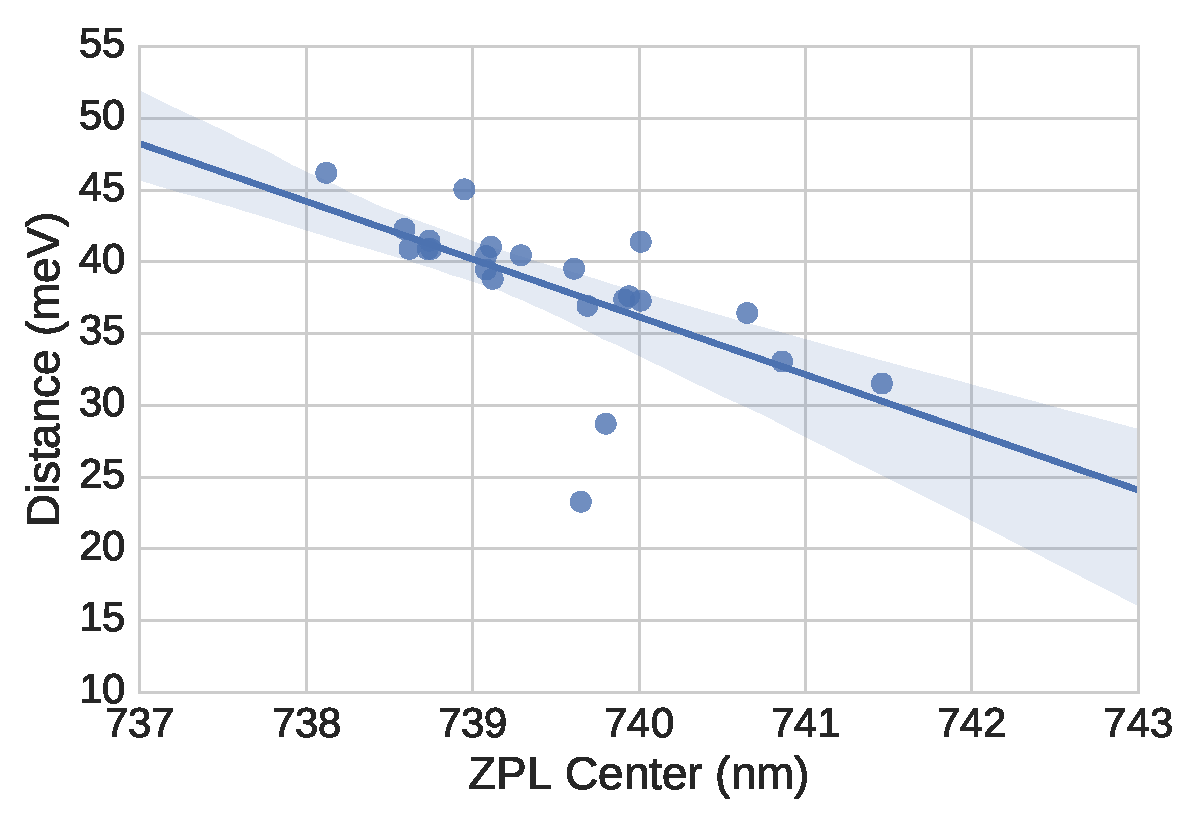
\includegraphics[trim = 0 0 0 0,  clip= true, width = 0.6\linewidth]{./pics/sideband_regression.pdf}}
			\caption[Shift of dominant side band peaks for \sivs]{Shift of dominant sideband peak from the \ZPL in spectra of \sivs (\vl, samples \insituF, \insituS, \insituH) vs. ZPL \cwl. The linear fit shows that the shift decreases with increasing ZPL center wavelength, i.e.\ with increasing strain and exhibits a slope of \SI[separate-uncertainty]{-4\pm1}{\milli\electronvolt\per\nano\meter}. The shaded area is the \SI{95}{\percent} confidence region.}
			\label{fig::sideband_fit}
		\end{figure}

		A recent study \cite{Londero2016} suggests that the \SI{42}{meV} mode, similar to other broad \psb features, originates from a resonance attributed to phonons causing the dynamical Jahn-Teller effect with \sivs \cite{Fu2009}.
		As the Jahn-Teller coupling varies with strain it is also expected that the resonance shifts accordingly.
		\\
		In the spectra of \vl, we do not observe a typical \siv sideband feature at \SI{64}{meV}, attributed to a local vibration of the \si atom, frequently much stronger than the  \SI{42}{meV} sideband peak.
		A possible explanation is, that the lattice mode at \SIrange{37}{43}{meV} is so strong that the local vibrational mode at \SI{64}{meV} cannot be separated from the tail of the lattice mode.
		% \\
		% \todo{beginning new}For further investigations, we plotted the \ZPL  of \vl with multiple peaks.
		% We found that two Lorentzian curves fit the peak best.
		% \Fref{fig::sideband_multfit} shows histograms of the distribution of the \cw and the \lw of the fitted peaks.
		% Keep in mind that two of the peaks sum up to the peak visible as a \ZPL and the third peak is the sideband peak which we attribute to the lattice mode at about \SI{43}{meV}.
		% We found that the \lw of the sideband peak exhibits values up to \SI{20}{nm}.
		% This broad width is an indicator, that the local vibrational mode might indeed be outpowered by the more intense lattice mode.
		% However, it is not very easy to find spectra where the sideband peak is pronounced and isolated enough to make proper statistics.
		% The original \ZPL is split up in two peaks, one with a median \cwl of \SI{738}{nm} (\SI{1680}{\meV}) and a median \lw of \SI{4.5}{nm}  and the other with a median \cwl of \SI{742}{nm} (\SI{1671}{\meV}) and a median \lw of \SI{8}{nm}.
		% It could be that this is an indication for another sideband peak with a shift of \SI{9}{\meV}.
		% \todo{end new}
		% \\
		% \begin{figure}[tp]
		% 	\begin{subfigure}[t]{ 0.49\linewidth}
		% 		\centering
		% 		\testbox{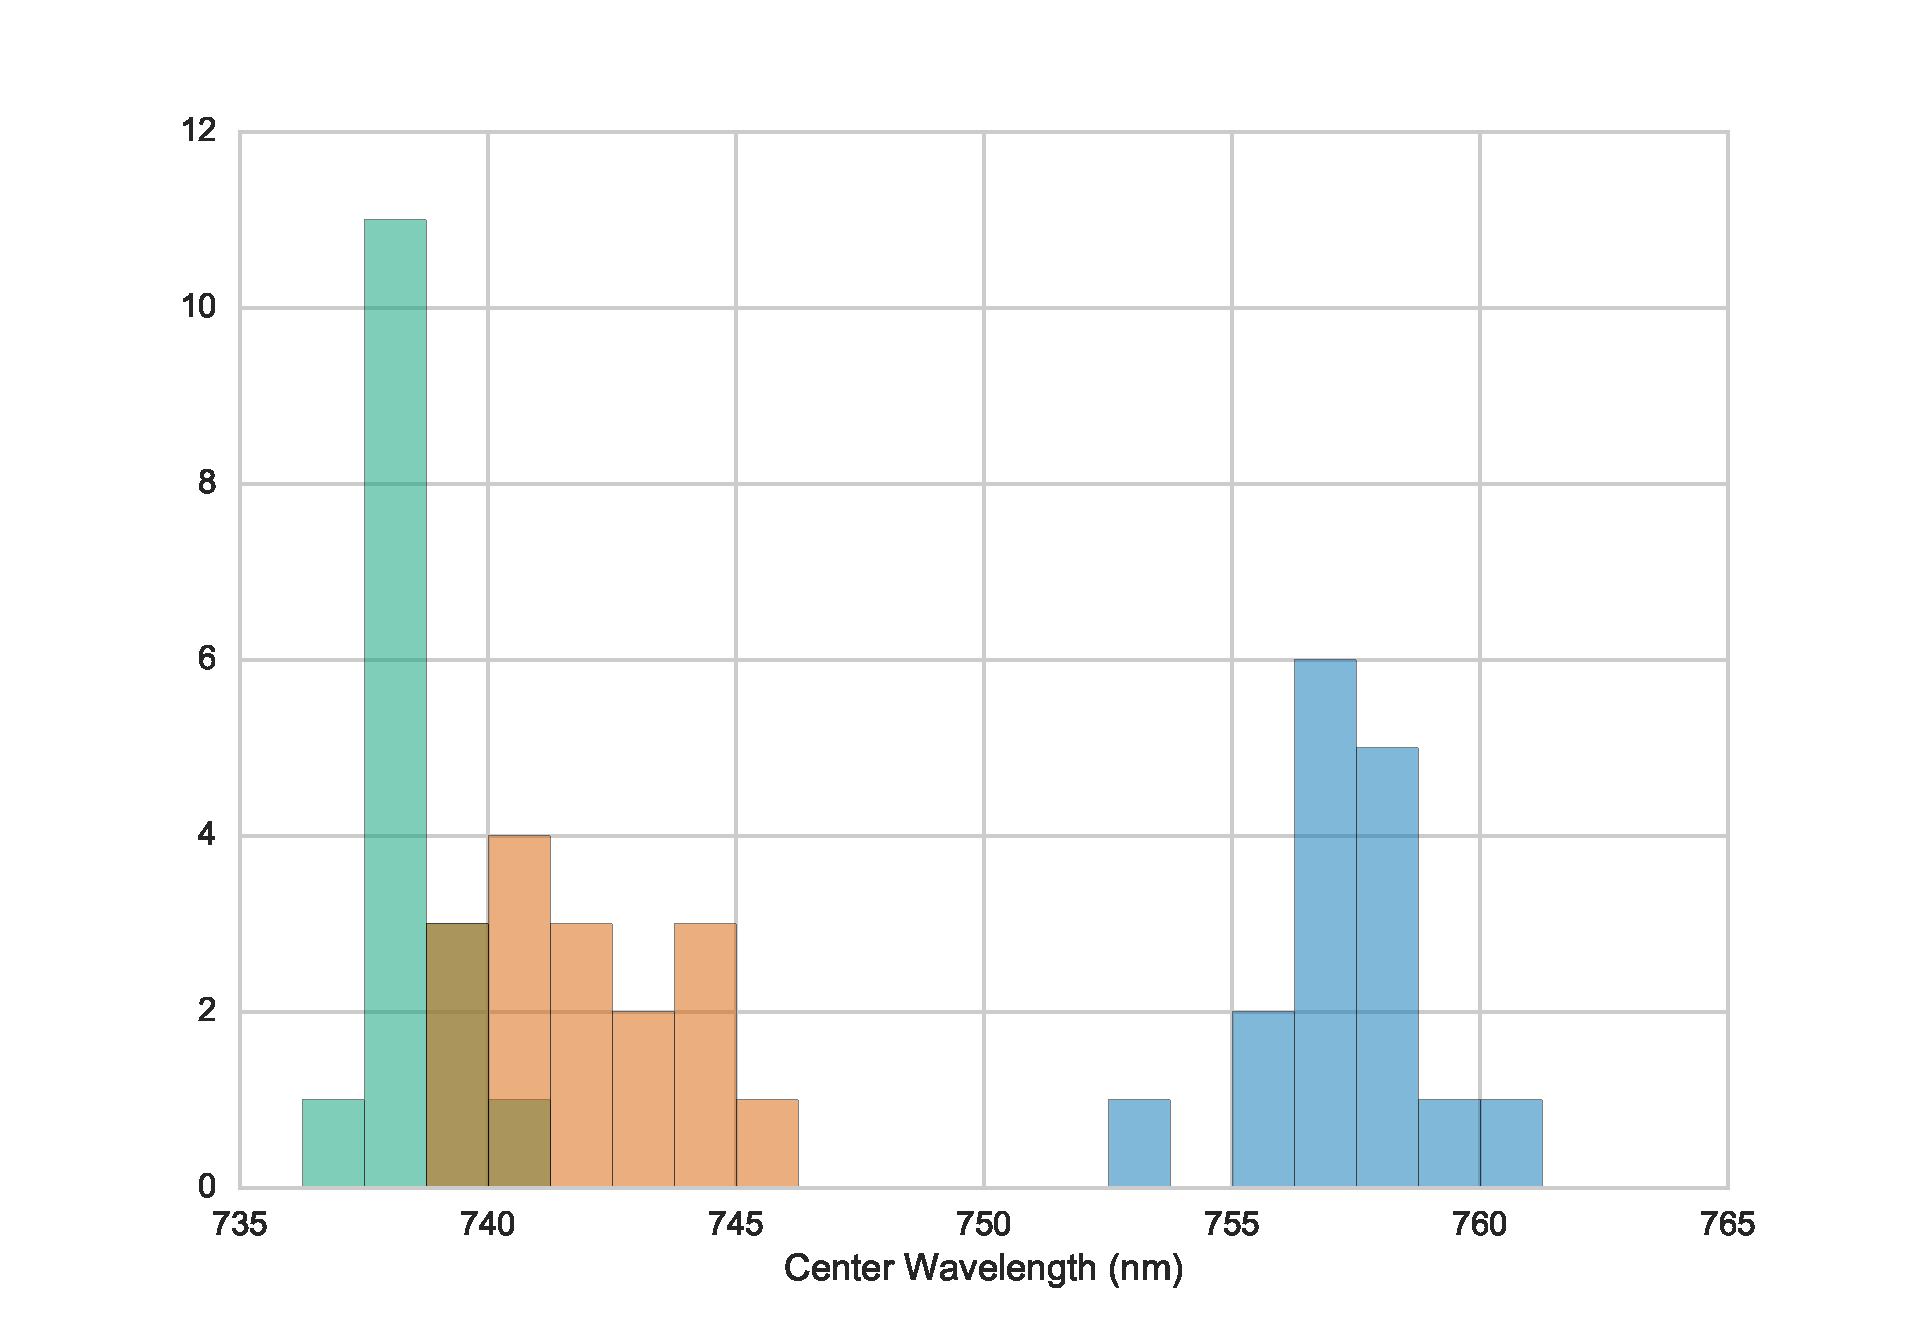
\includegraphics[trim = 0 0 0 0,  clip= true, width = \textwidth]{./pics/histo_multi_sidebands_position25bins.pdf}}
		% 		\caption{}
		% 		\label{subfig::sb_multfit_pos}
		% 	\end{subfigure}
		% 	\hfill
		% 	\begin{subfigure}[t]{ 0.49\linewidth}
		% 		\centering
		% 		\testbox{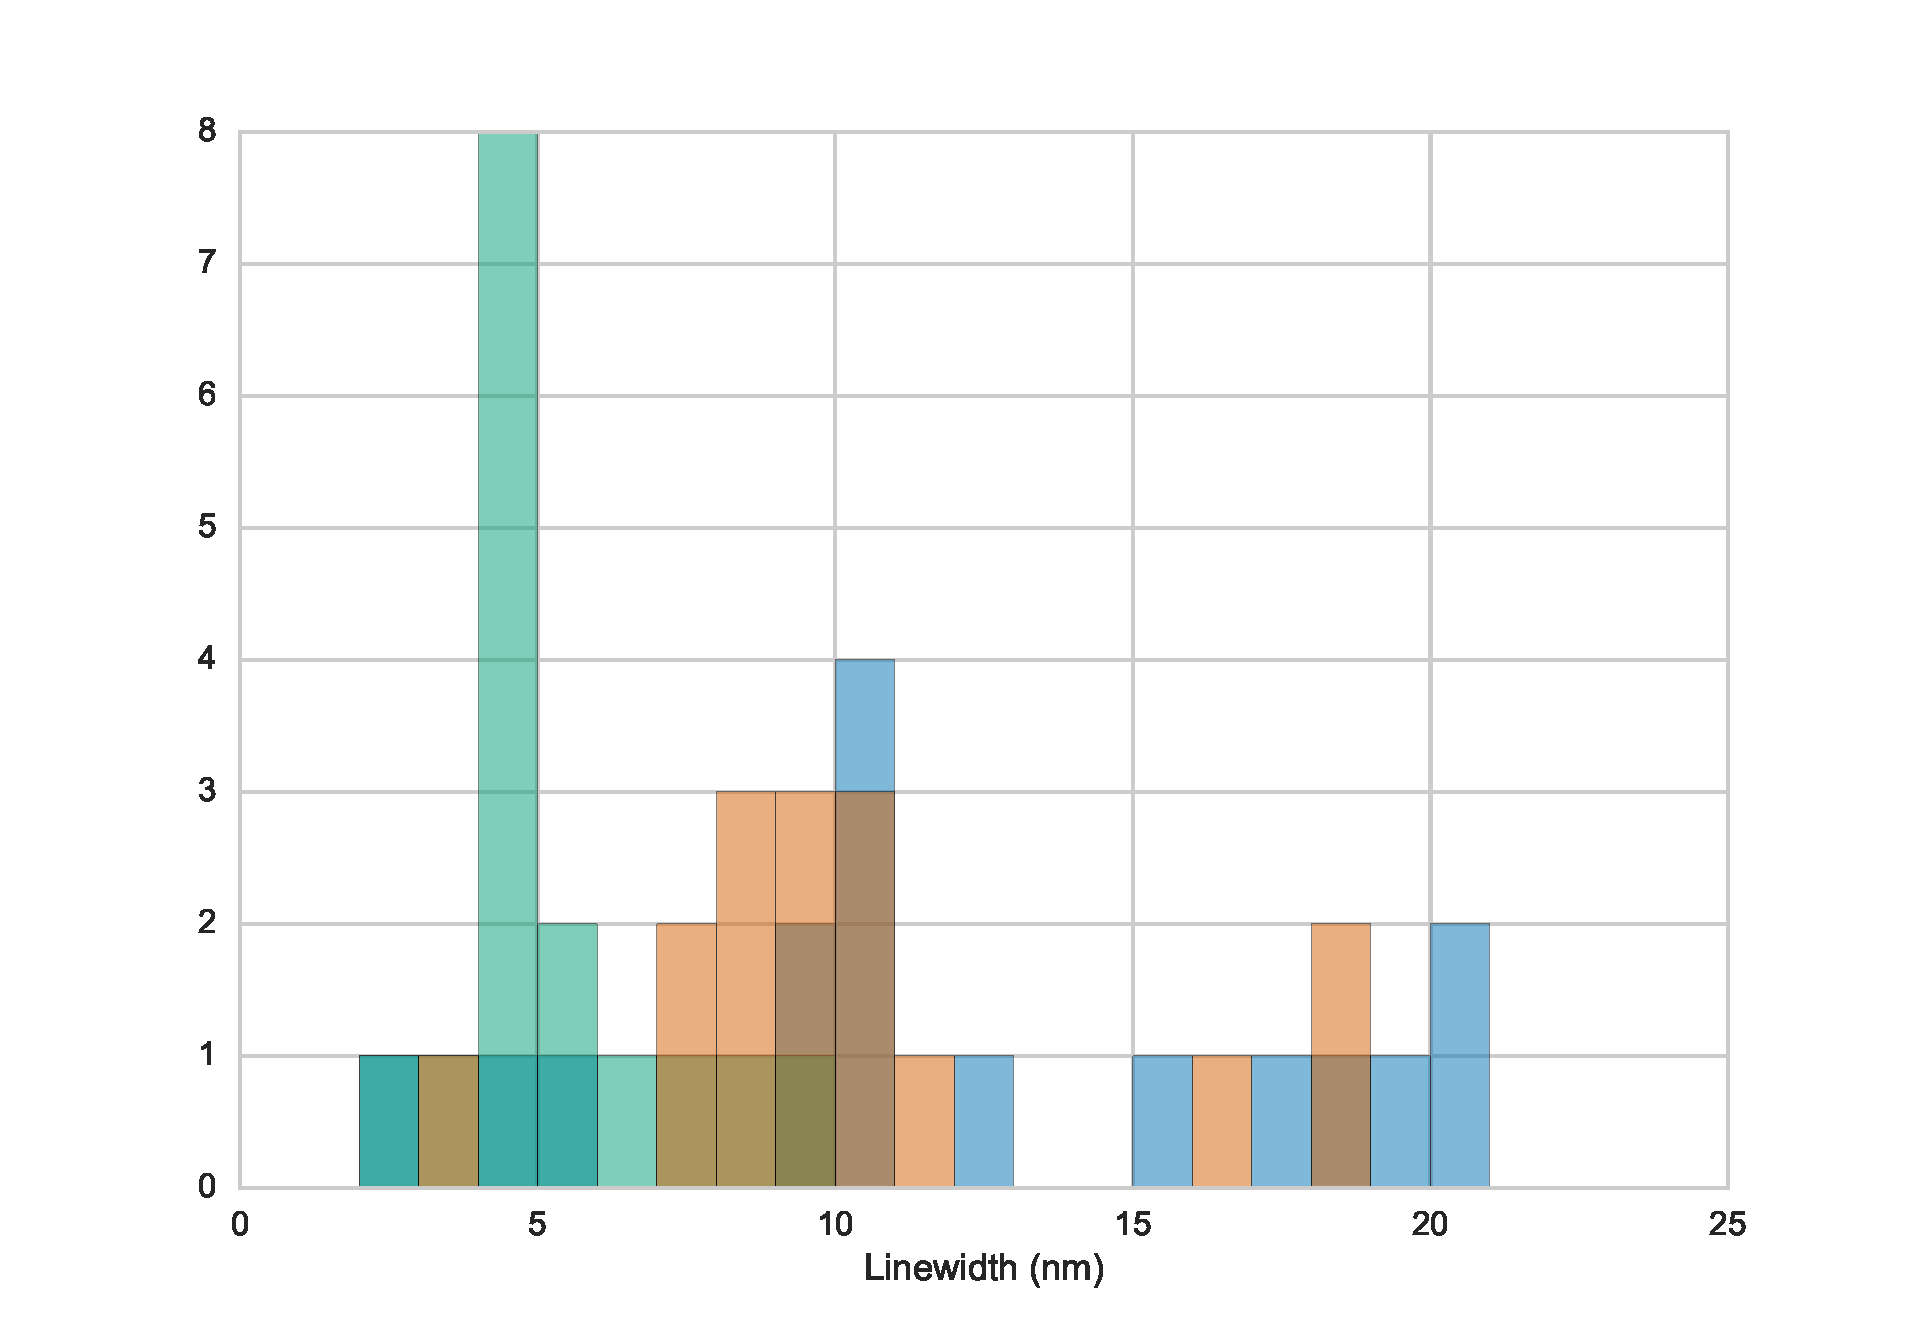
\includegraphics[trim = 0 0 0 0,  clip= true, width = \textwidth]{./pics/histo_multi_sidebands_width_25bins.pdf}}
		% 		\caption{}
		% 		\label{subfig::sb_multfit_width}
		% 	\end{subfigure}
		% 	\caption{}
		% 	\label{fig::sideband_multfit}
		% \end{figure}
		% \\
		In \hl we observe many spectra which exhibit several peaks within the spectral range of our detection range between \SIrange{710}{900}{nm}.
		The challenge arises to unequivocally distinguish between peaks stemming from a phonon sideband and peaks stemming from shifted, less intense \siv \ZPLs.

		Interestingly, we assert a tendency for peaks to accumulate at a shift of around \SIlist{43;64;150;175}{meV}, as shown in \Fref{fig::multiple_sb_peaks}. This pattern in the \psb of \hl is consistent with side band shifts reported in \cite{Sternschulte1994,Zaitsev2000, Neu2011}.

		\begin{figure}[!htb]
			\centering
			\testbox{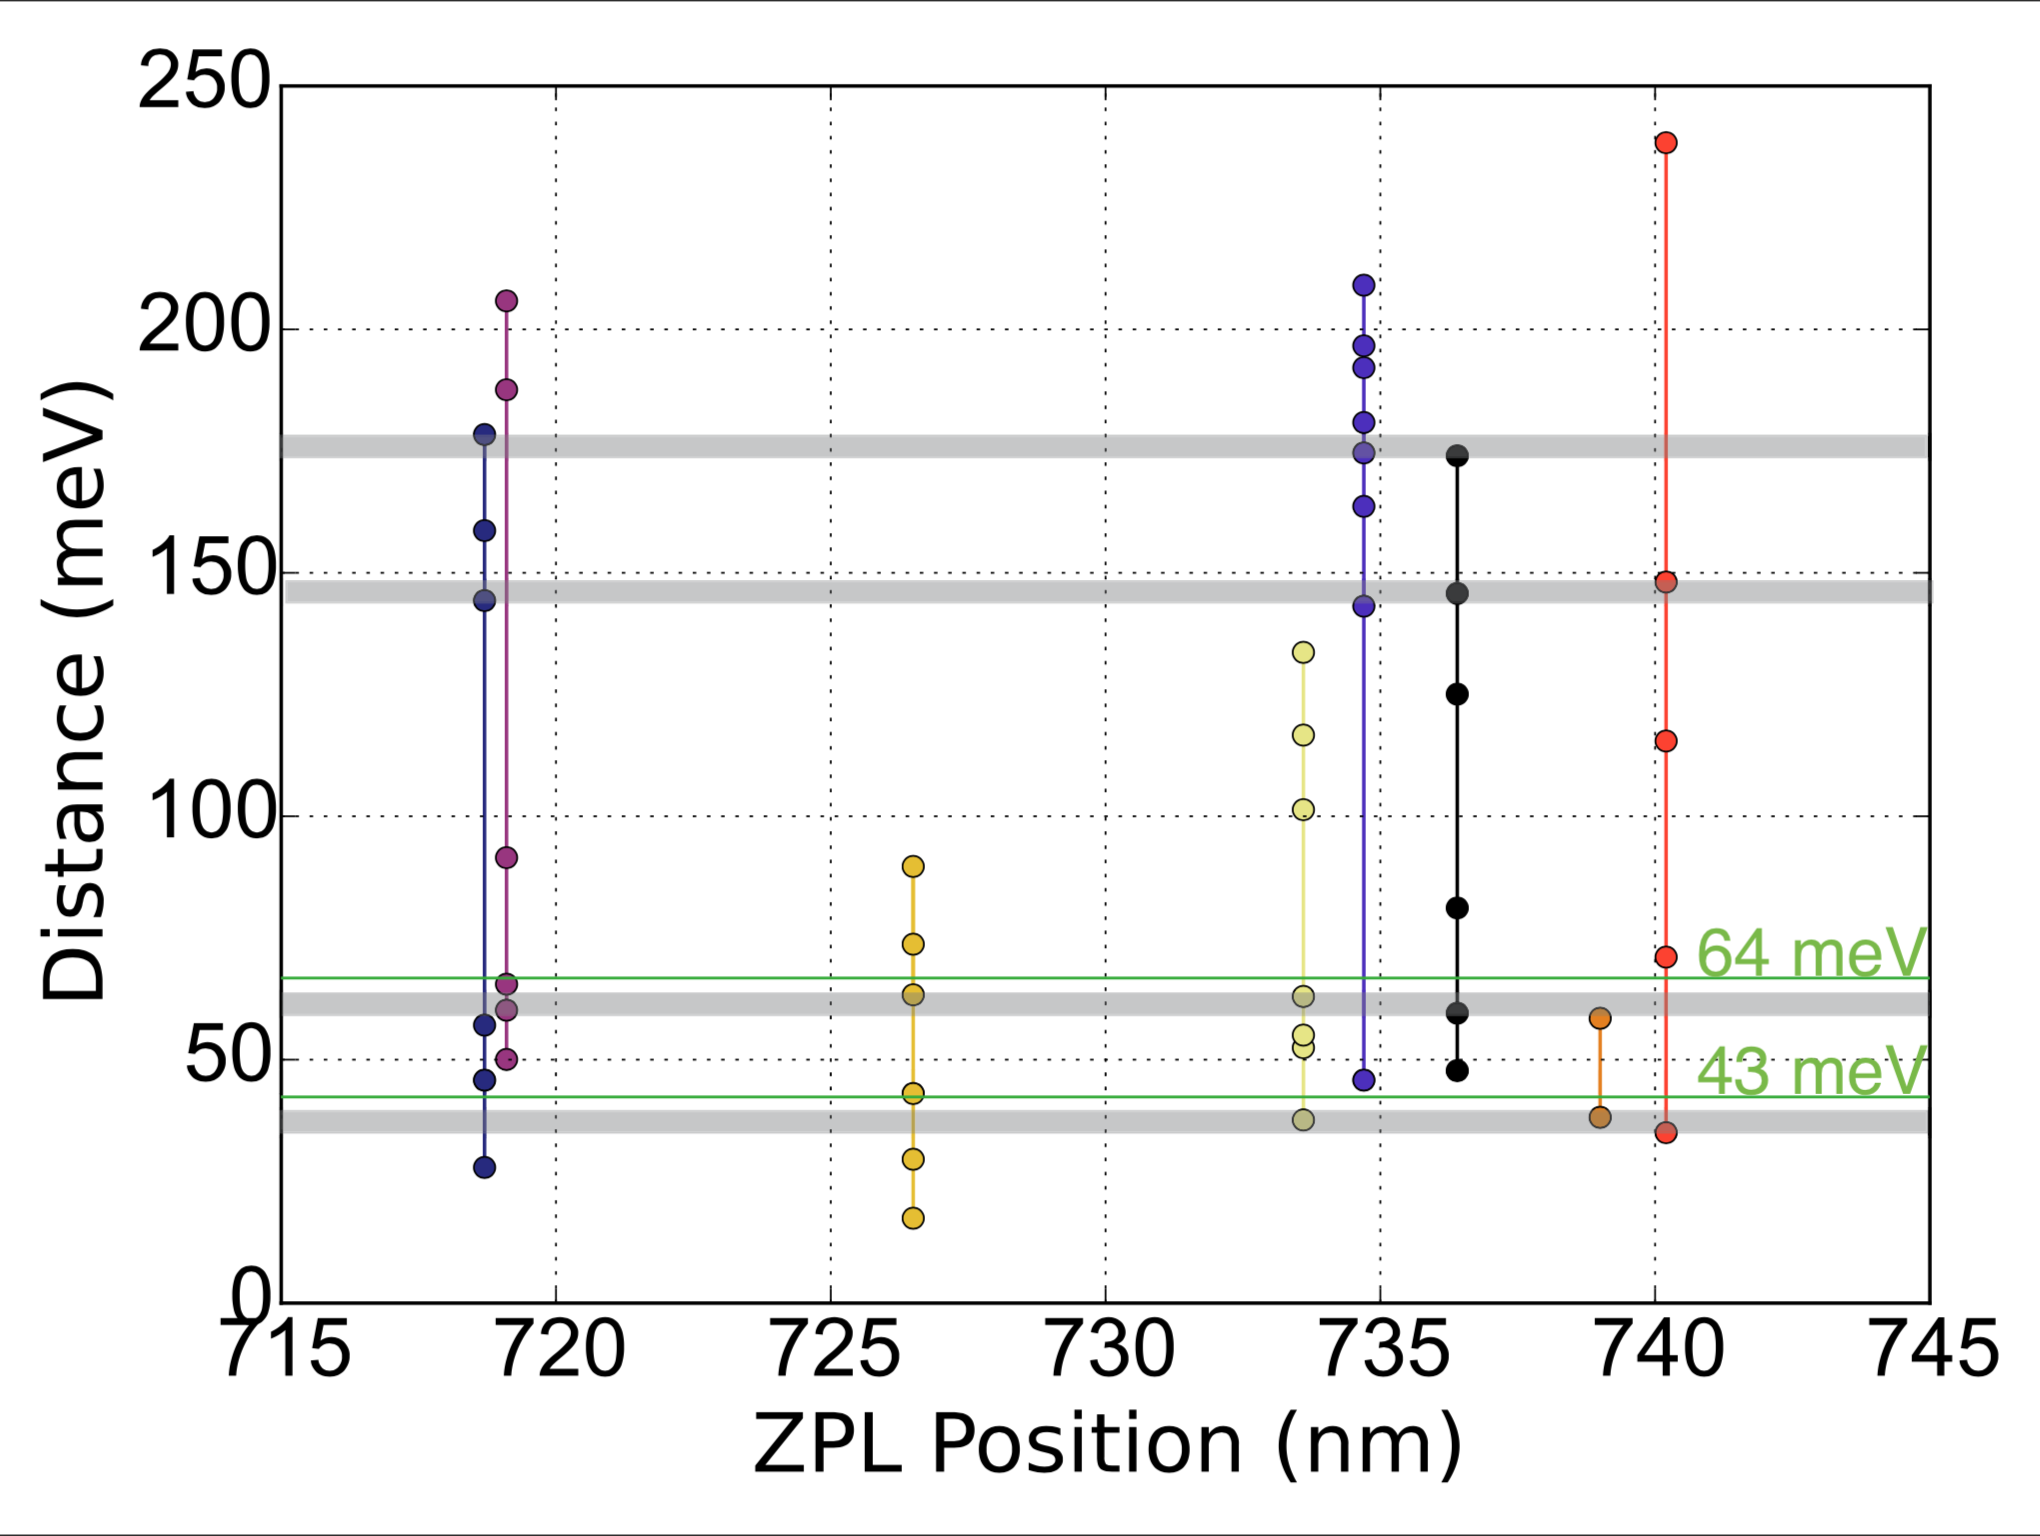
\includegraphics[trim = 0 0 0 0,  clip= true, width = 0.6\linewidth]{./pics/statistics_only_multiple_sb_zpl_vs_distance_5meVbars_modes_edit.png}}
			\caption[Accumulation of sideband peaks]{This plots shows sideband peaks attributed to different \ZPL \cwls, with respect to the sideband peak's shift. The \ZPL \cwl is visualized on the x-axis, the respective sideband peak shifts on the y-axis. Therefore, data points aligned on a vertical line belong to the same spectrum. For better visibility, all data points of one spectrum are colored in the same color. Areas shaded in grey represent an accumulation of sideband shifts. The green lines indicate distances with \SI{43}{meV} and \SI{64}{meV} respectively.}
			\label{fig::multiple_sb_peaks}
		\end{figure}

		The possibility exists, that some these peaks believed to be \psbs are actually shifted \ZPLs stemming from other \sivs. To address this question, we perform \pl measurements at cryogenic temperatures.


		\subsection{Cryostatic Measurements}\label{subsec::cryo}

			\begin{figure}[!htb]
				\begin{subfigure}[t]{ 0.49\linewidth}
					\centering
					\testbox{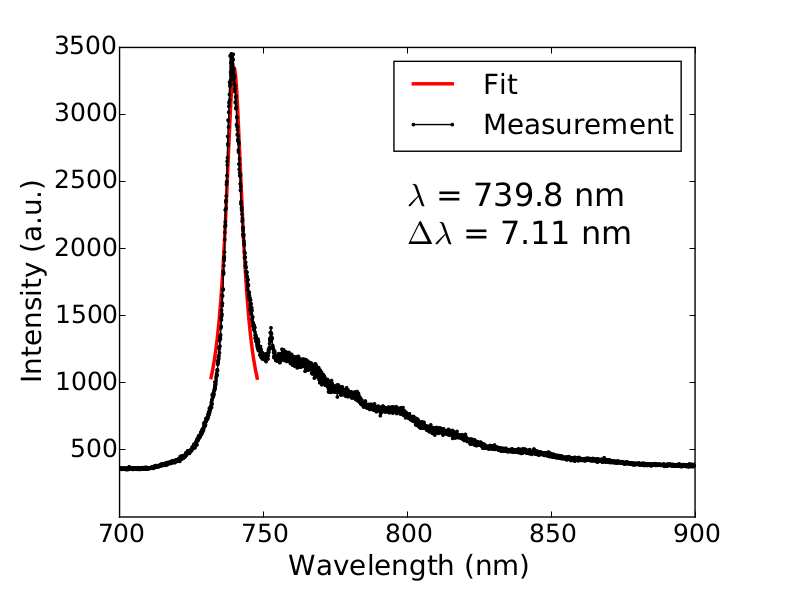
\includegraphics[trim = 0 0 0 0,  clip= true, width = \pairplotwide]{./pics/Ir25Mox_fit_spe_scan_xy-08x11y19_297uW_t180.png}}
					\caption{}
					\label{subfig::roomtep1}
				\end{subfigure}
				\hfill
				\begin{subfigure}[t]{ 0.49\linewidth}
					\centering
					\testbox{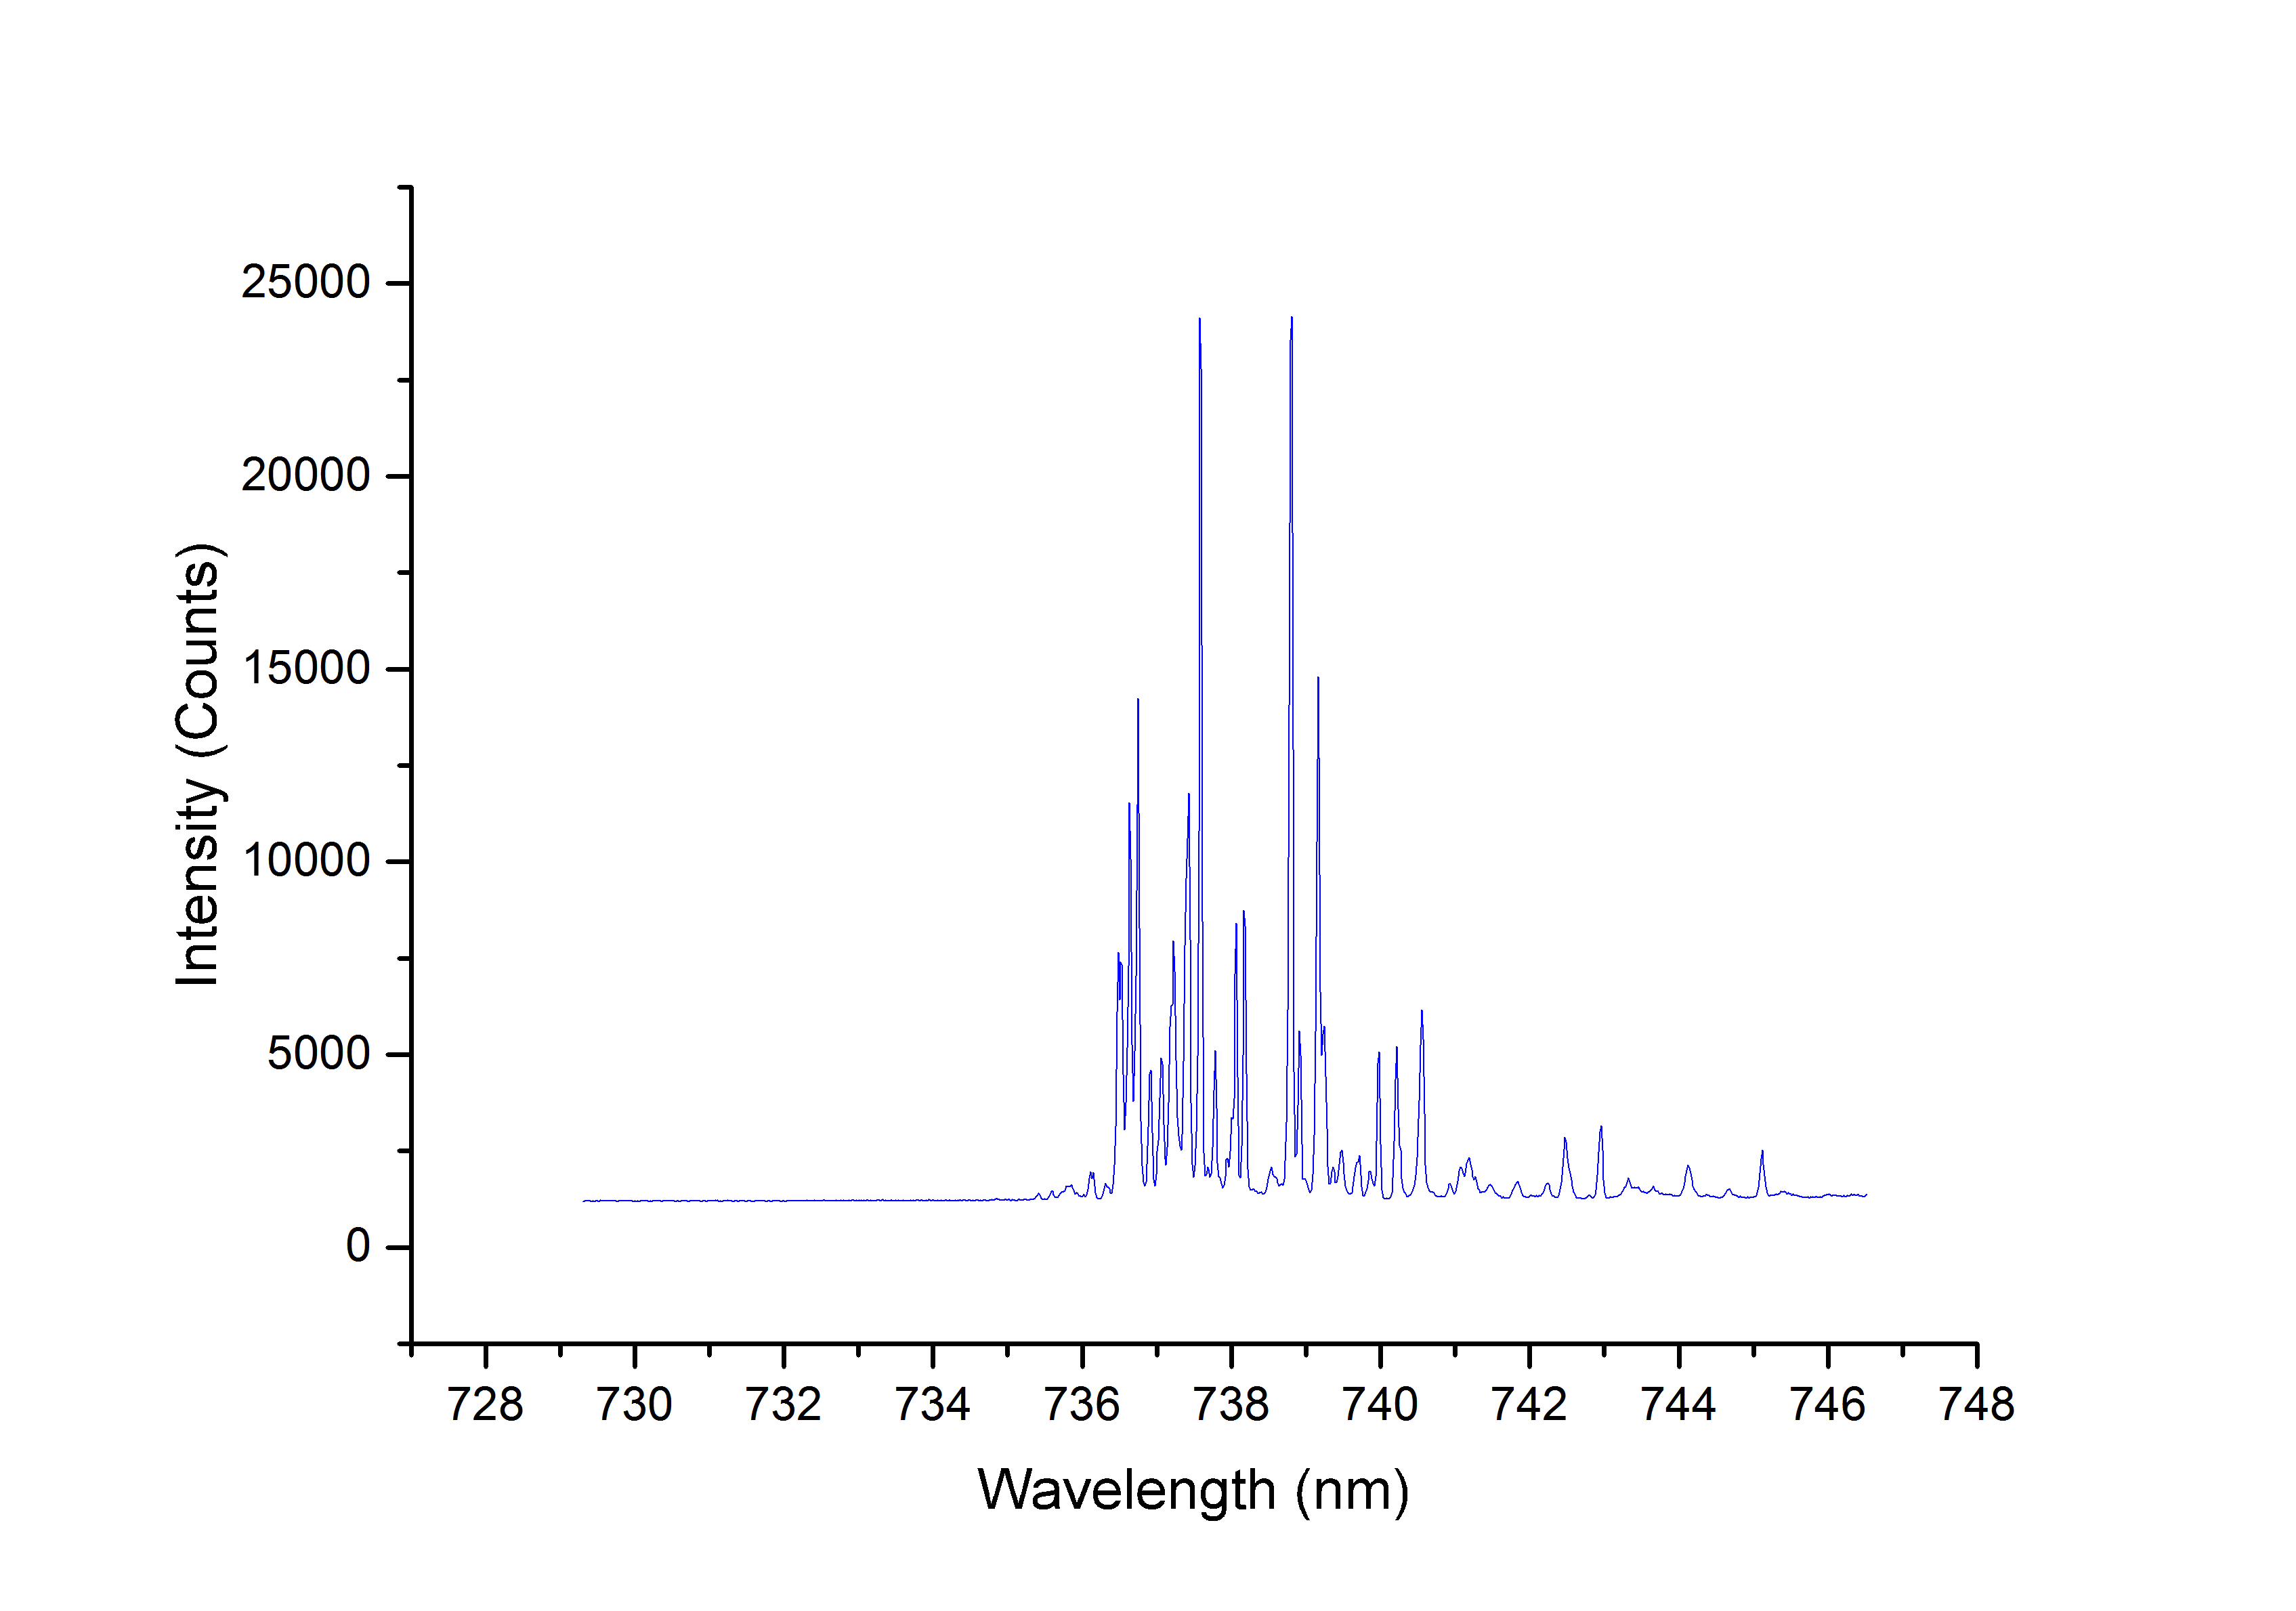
\includegraphics[trim = 0 0 0 0,  clip= true, width = \pairplotwide]{./pics/cryo_Spektrum68_edit.png}}
					\caption{}
					\label{subfig::cryo1}
				\end{subfigure}
				\hfill
				\begin{subfigure}[t]{ 0.49\linewidth}
					\centering
					\testbox{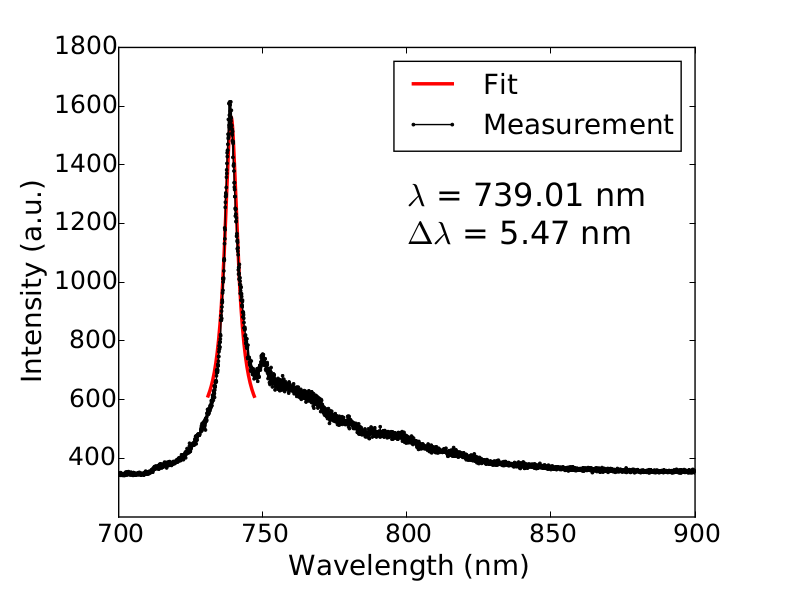
\includegraphics[trim = 0 0 0 0,  clip= true, width = \pairplotwide]{./pics/Ir25M_rt_to_cryo_84_fit_spe_scan_xy-35x10y12_300uW_t120.png}}
					\caption{}
					\label{subfig::roomtep2}
				\end{subfigure}
				\hfill
				\begin{subfigure}[t]{ 0.49\linewidth}
					\centering
					\testbox{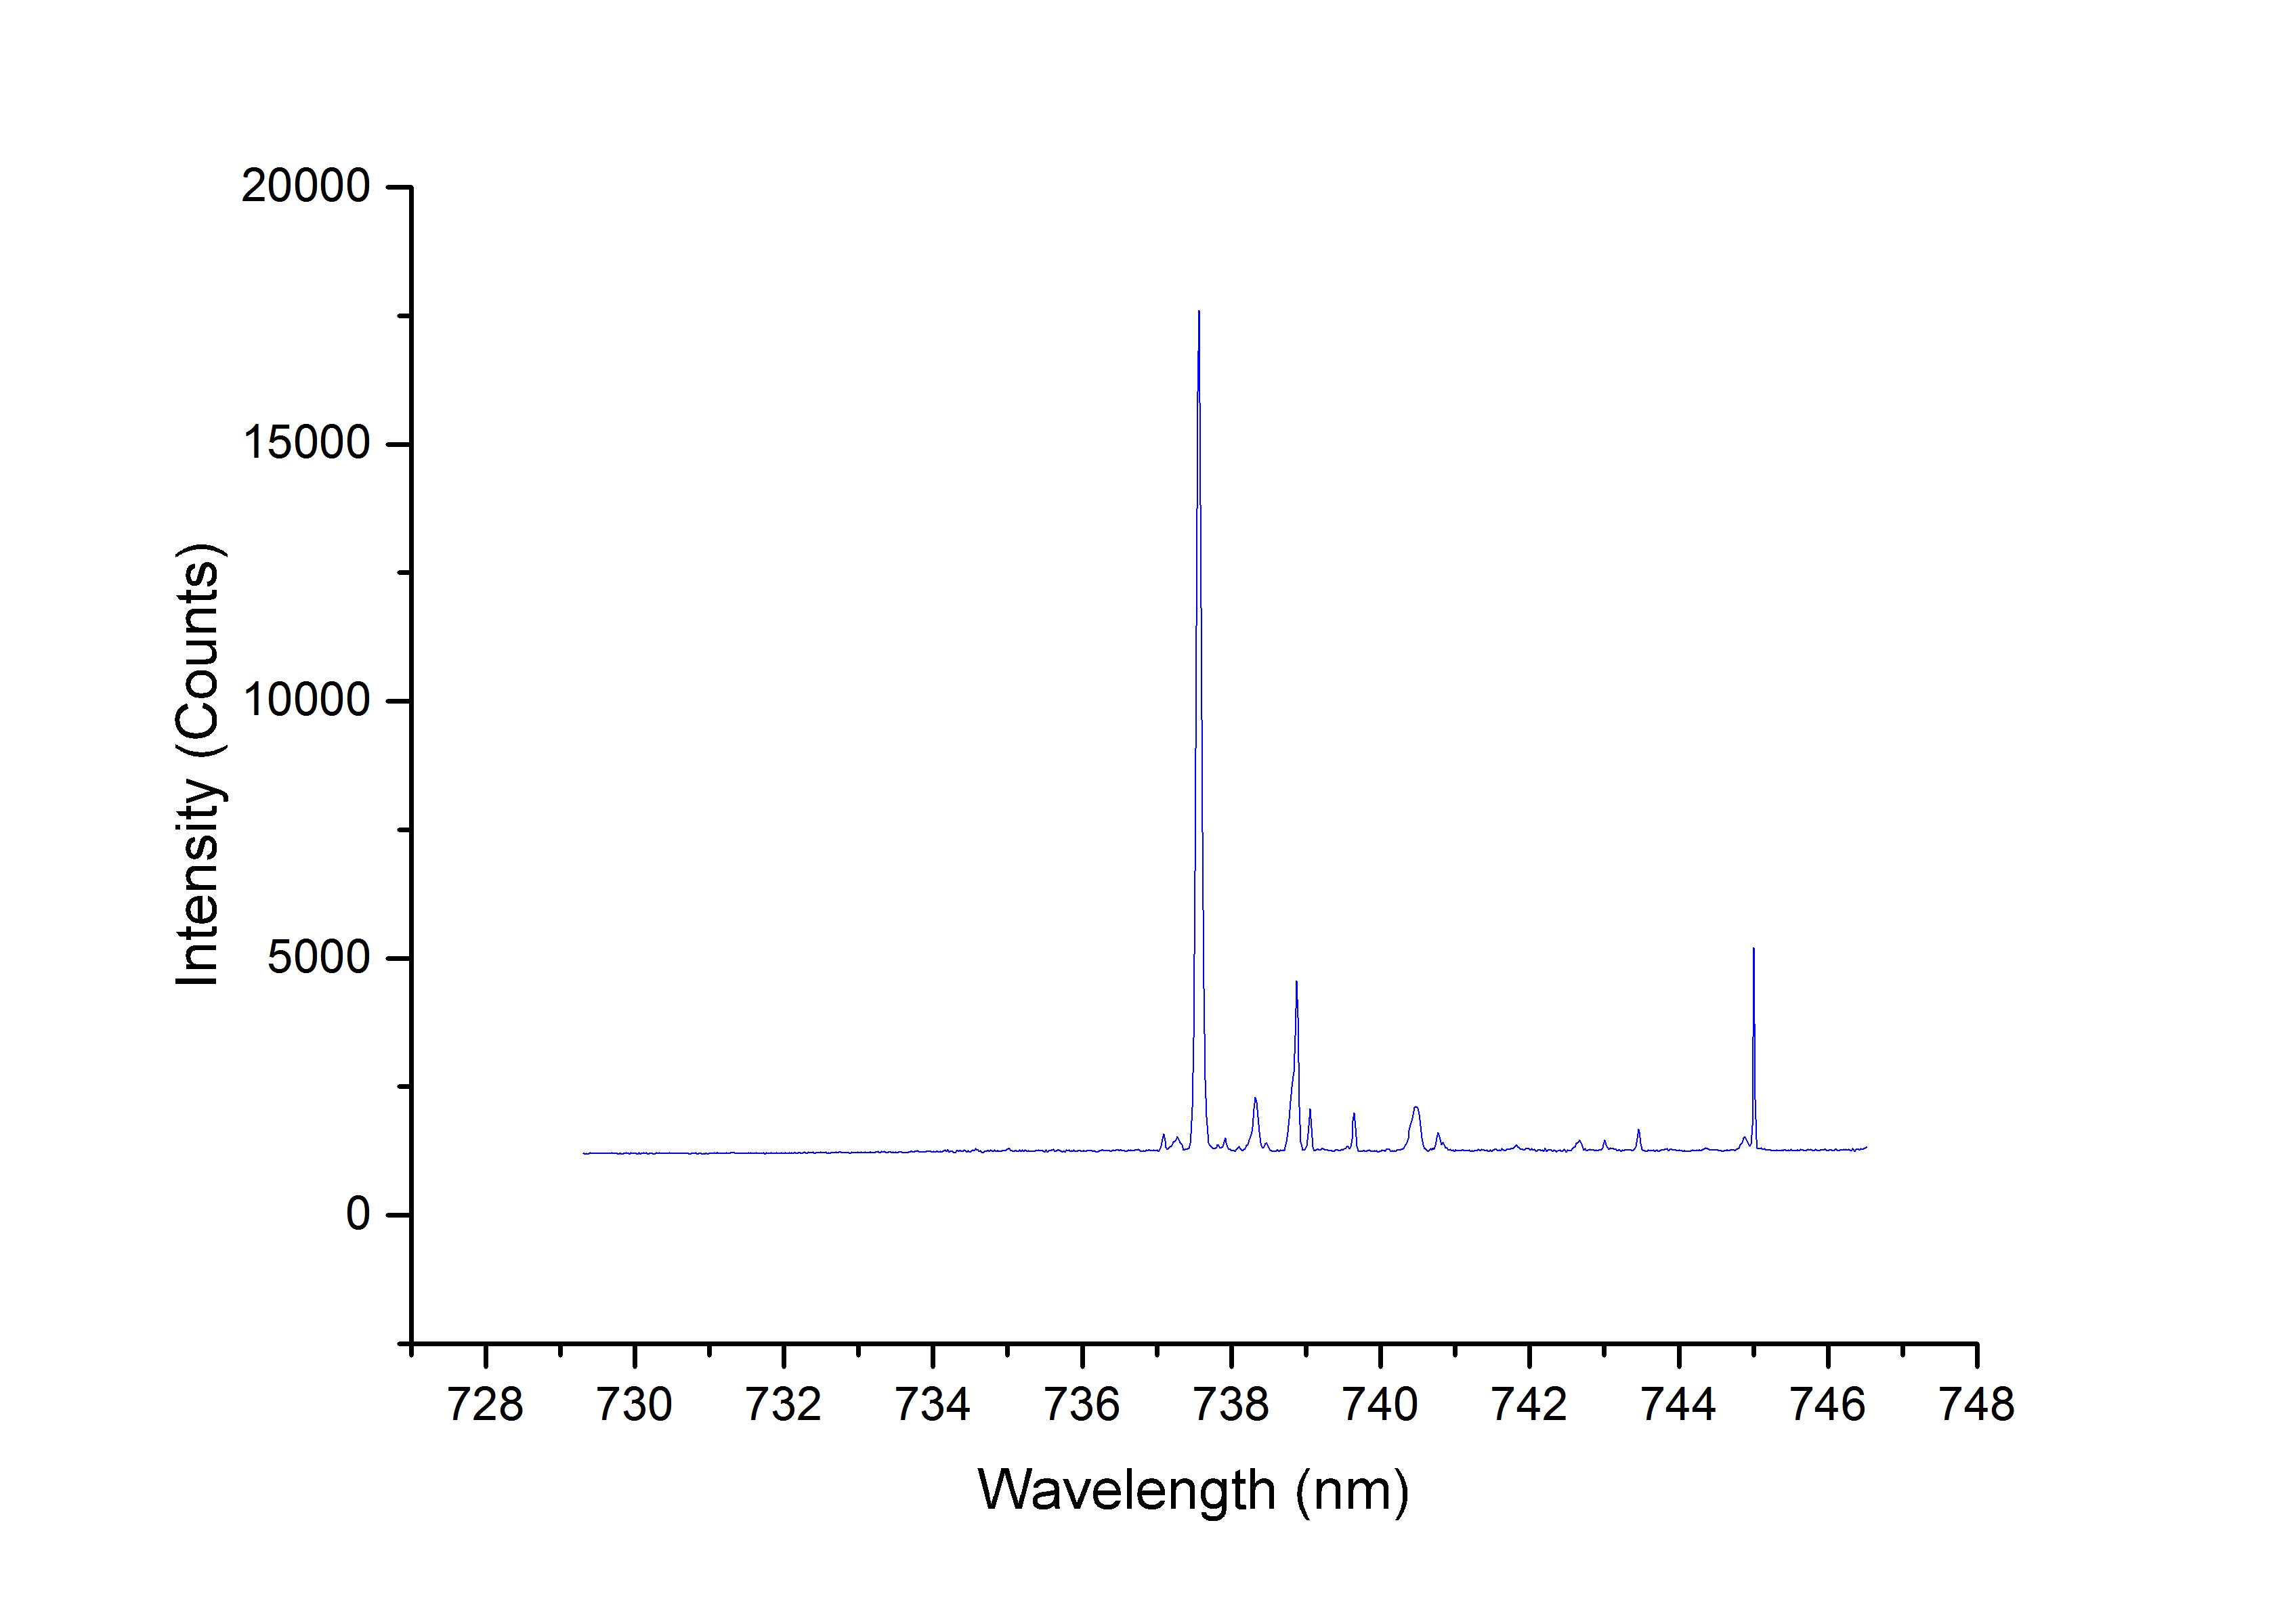
\includegraphics[trim = 0 0 0 0,  clip= true, width = \pairplotwide]{./pics/cryo_Spektrum84_edit.png}}
					\caption{}
					\label{subfig::cryo2}
				\end{subfigure}
				\caption[Spectra of \nds at cryogenic temperatures]{Comparison of spectra taken at room-temperature (l.h.s) and at cryogenic temperatures (r.h.s). At low temperatures a multitude of lines is revealed indicating several \sivs embedded in a strained lattice neighborhood.}
				\label{fig::rt_vs_cryo}
			\end{figure}

			At cryogenic temperatures \psb contributions vanish, allowing a focused investigation of \zpls.
			In particular, for \sivs a four-way splitting of the \zpl is expected, see \Fref{ch::introduction}.
			To conduct low-temperature measurements, we used a confocal setup similar to the one described in \Fref{ch::pl_setup}.
			It differs merely by the fact that the sample is efficiently cooled to \SI{4}{\kelvin} using a cryostat.
			\\
			In \Fref{fig::rt_vs_cryo} measurements of two individual \nds are shown, both situated on sample \insituSo.
			\Fref{subfig::cryo1} and \Fref{subfig::cryo2} show spectra recorded at cryogenic temperatures while \Fref{subfig::roomtep1} and \Fref{subfig::roomtep2} show spectra recorded at room temperature for comparison.
			Instead of the four-fold degeneracy expected for \sivs in low-strain diamond, the cryogenic measurements indicate a multitude of various lines.
			The observation is best explained by the presence of several \sivs which are subject to varying levels of strain in their local lattice neighborhood.
			Given the fact that \zpls are found spread over a significant range of \wls, a non-negligible impact of lattice strain on \siv luminescence is revealed.
